\documentclass[12pt,a4paper]{article} 
\usepackage[portuguese]{babel} \usepackage[utf8]{inputenc}
\usepackage{amsmath} 
\usepackage{graphicx}
\usepackage{booktabs}
\usepackage{pgfplots}
\usepackage{tikz}
\usepackage{float}
\pgfplotsset{compat=1.15}
\begin{document}
\setcounter{figure}{1}
\setcounter{section}{2}
\setcounter{page}{6}
\section{Relatório}
\subsection{Introdução}

Nesta prática, deseja-se entender o funcionamento  do efeito da polarização 
automática no ponto de operação de transistores; prática essencial para a realização 
de projetos de circuitos discretos.\\

\begin{figure}[htpb]
  \centering
  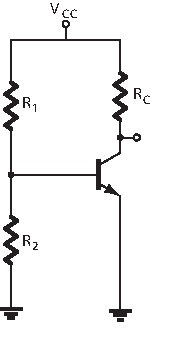
\includegraphics[width=0.3\linewidth]{./img/divisortensao.pdf}
  \caption{Arranjo do circuito para que a polarização automática ocorra através de um divisor de tensão.}
  \label{fig:divisortensao}
\end{figure}

A polarização do circuito advém da necessidade de estabelecer uma corrente contínua 
constante no emissor do transistor. Neste experimento, 
utilizaremos uma configuração de emissor comum (transistor bipolar \emph{NPN}); que apresenta um ganho de corrente, 
tensão e potência elevados aliados a resistência de entrada baixa
e resistência de saída alta. Esta configuração será polarizada usando um divisor de tensão,
que garantirá uma tensão e corrente de polarização,
$V_{CEq}$ e $I_{Cq}$, independentes do ganho de corrente, $\beta$, do transistor.
Tal indepência é conveniente, pois $\beta$ 
não é um valor bem definido na fabricação e é muito sensível a variações na temperatura.
No entanto, deve-se escolher um ponto de polarização, $Q$, adequado que permita a 
máxima excursão do sinal de saída.

\begin{figure}[htpb]
  \centering
  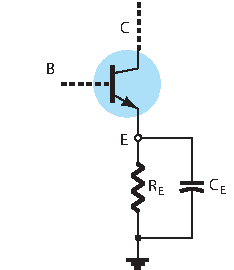
\includegraphics[width=0.35\linewidth]{./img/bypass.pdf}
  \caption{Capacitor \emph{bypass}, $C_e$, utilizado no emissor de um circuito com transistor bipolar.  }
  \label{fig:.ext}
\end{figure}

A importância de capacitores de ``bypass'' e de acoplamento também devem ser ressaltados.
Capactiores de acoplamento são necessários para garantir que uma entrada, com nível DC
qualquer, possa ser separada do sinal AC da entrada, garantindo que apenas correntes 
alternadas componham o sinal de entrada do circuito. \\
Capacitores de ``bypass'' atuam como filtros para componentes AC que possam estar 
presentes no sinal DC, garantindo um sinal de DC mais puro e limpo.
Sabemos que para sinais de baixas frequências, o capacitor 
tem uma alta resistência; desta forma sinais de baixa frequência não passarão por ele
(correntes tendem a ir para o caminho que oferece menor resistência). De forma contrária,
também sabemos que capacitores oferecem baixíssimas resistências em altas frequências (
como nosso sinal AC de entrada), o que levará a um curto circuito entre o emissor e o terra,
nos fazendo desprezar a resistência conectada ao emissor. \\
Se retiramos o capacitor de ``bypass'' do circuito, teremos um circuito 
chamado de emissor comum degenerado. Este novo circuito apresentaum ganho muito menor em
relação ao emissor comum degenerado, fato que iremos comprovar durante esta prática.


\subsection{Análises}
Calculou-se os valores ideais para as resistências do circuito mostrado pela Figura~1, 
cálculos presentes no item 1 da seção 2.2.  Estes valores foram adequados a valores 
comerciais de resistência. A partir dos valores comerciais, pode-se por fim, estimar 
as correntes ideias que devem  passar pelo transistor. Testou-se 
se os transistores estavam operando de forma correta, através da função diodo do multímetro
digital. 
\begin{table}[htpb]
  \centering
  \caption{Valores de resistência idealizados para o projeto, comerciais e os valores, de fato, medidos.}
  \label{tab:label}

  \begin{tabular}{c c c c}
    \\  \toprule 
    & Ideal $(\Omega)$ &Comercial $(\Omega)$  & Medido$(\Omega)$\\ \midrule
    $R_{c}$ & 667 &680 & 674 \\ \midrule
    $R_1$   &11.3k  &12k & 11.88k \\ \midrule
    $R_2$   &3.89k  &3.9k &3.82k \\ \bottomrule
  \end{tabular}
\end{table}
\begin{table}[htpb]
  \centering
  \caption{Valores estimados de tensão e corrente no transistor e valores empiricamente obtidos.}
  \label{tab:transvalues}
  \begin{tabular}{c c c c c}
    \\  \toprule
    & $V_{RC} (V)$ & $V_{CE} (V) $ & $V_{RE} (V)$  \\ \midrule
    Estimados  & 6.28         & 5.72          & 3.14          \\ \midrule
    BC-237 (1) & 5.76         & 6.23          & 2.90         \\ \midrule
    BC-237 (2) & 5.68         & 6.27          & 2.87          \\ \midrule
    BC-547     & 5.61         & 6.39          & 2.83          \\ \bottomrule
  \end{tabular}
\end{table}
\begin{table}[htpb]
  \centering
  \caption{Ganho do circuito teórico comparado com o ganho empírico de diversos transistores.}
  \label{tab:ganho}
  \begin{tabular}{c c c c c}
    \\ \toprule 
    & $I_{B} (mA)$ & $I_{C} (mA)$ & Ganho  & Ganho (dB) \\ \midrule
    Estimados  & 0.05         & 9.32         & 186.4  & 45.4 \\ \midrule
    BC-237 (1) & 0.016        & 8.53         & 533.13 & 54.53 \\ \midrule
    BC-237 (2) & 0.0152       & 8.42         & 553.95 & 54.87 \\ \midrule
    BC-547     & 0.032        & 8.32         & 260    & 48.30 \\ \bottomrule

  \end{tabular}
\end{table}
\begin{table}[htpb]
  \centering
  \caption{Ganhos téoricos e experimentais referentes ao experimento 2, com um 
    entrada senoidal.}
  \label{tab:Ganho}
  \begin{tabular}{c c c c}
    \\ \toprule
    & Ganho teórico & Ganho experimental& Erro ($\%$)\\ \midrule
    Não Degenerado & -243.3 & -150 & 34.2  \\ \midrule
    Degenerado & -1.57 & -1.3 & 23.0 \\ \bottomrule
  \end{tabular}
\end{table}
Em seguida, montou-se o circuito da Figura~1 e, aplicado apenas um sinal DC, 
mediu-se as correntes e tensões do transistor bipolar. 
Comparou-se os valores reais e os obtidos em projeto, variando 
o transistor por um mesmo de mesmo modelo , \emph{BC-247}, e por outro de 
modelo diferente, \emph{BC-547}, repetindo o procedimento anterior.

No experimento seguinte, adicionamos um sinal de amplitude baixa, desta vez com um capacitor de \emph{bypass}
conectado na entrada, e observamos o ganho que o circuito apresentou em sua saída. Em seguida, 
a fim de perceber a influência do capacitor no ganho, retiramos este e observamos sua forma de onda.
\begin{figure}[htpb]
  \centering
  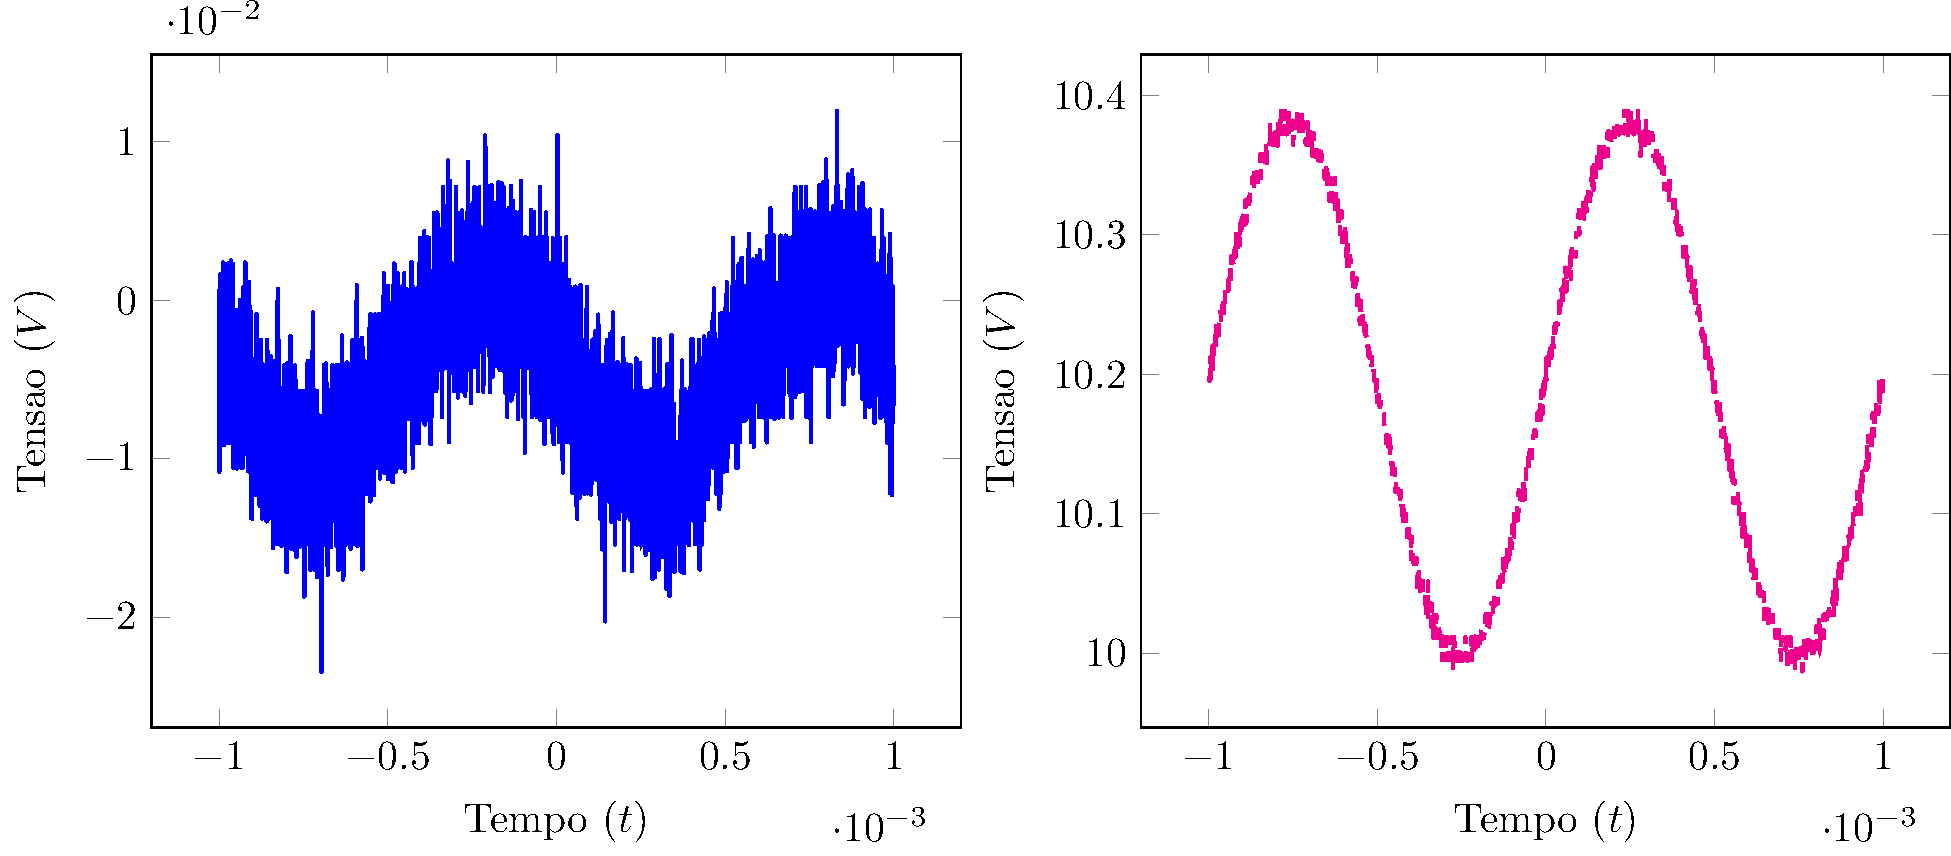
\includegraphics[width=\linewidth]{./img/scope1.pdf}
  \caption{Tensão de entrada (1Khz), em azul, e tensão de saída, magenta, do circuito representado na Figura~1.}
  \label{fig:ndegenerado}
\end{figure}
\begin{figure}[htpb]
  \centering
  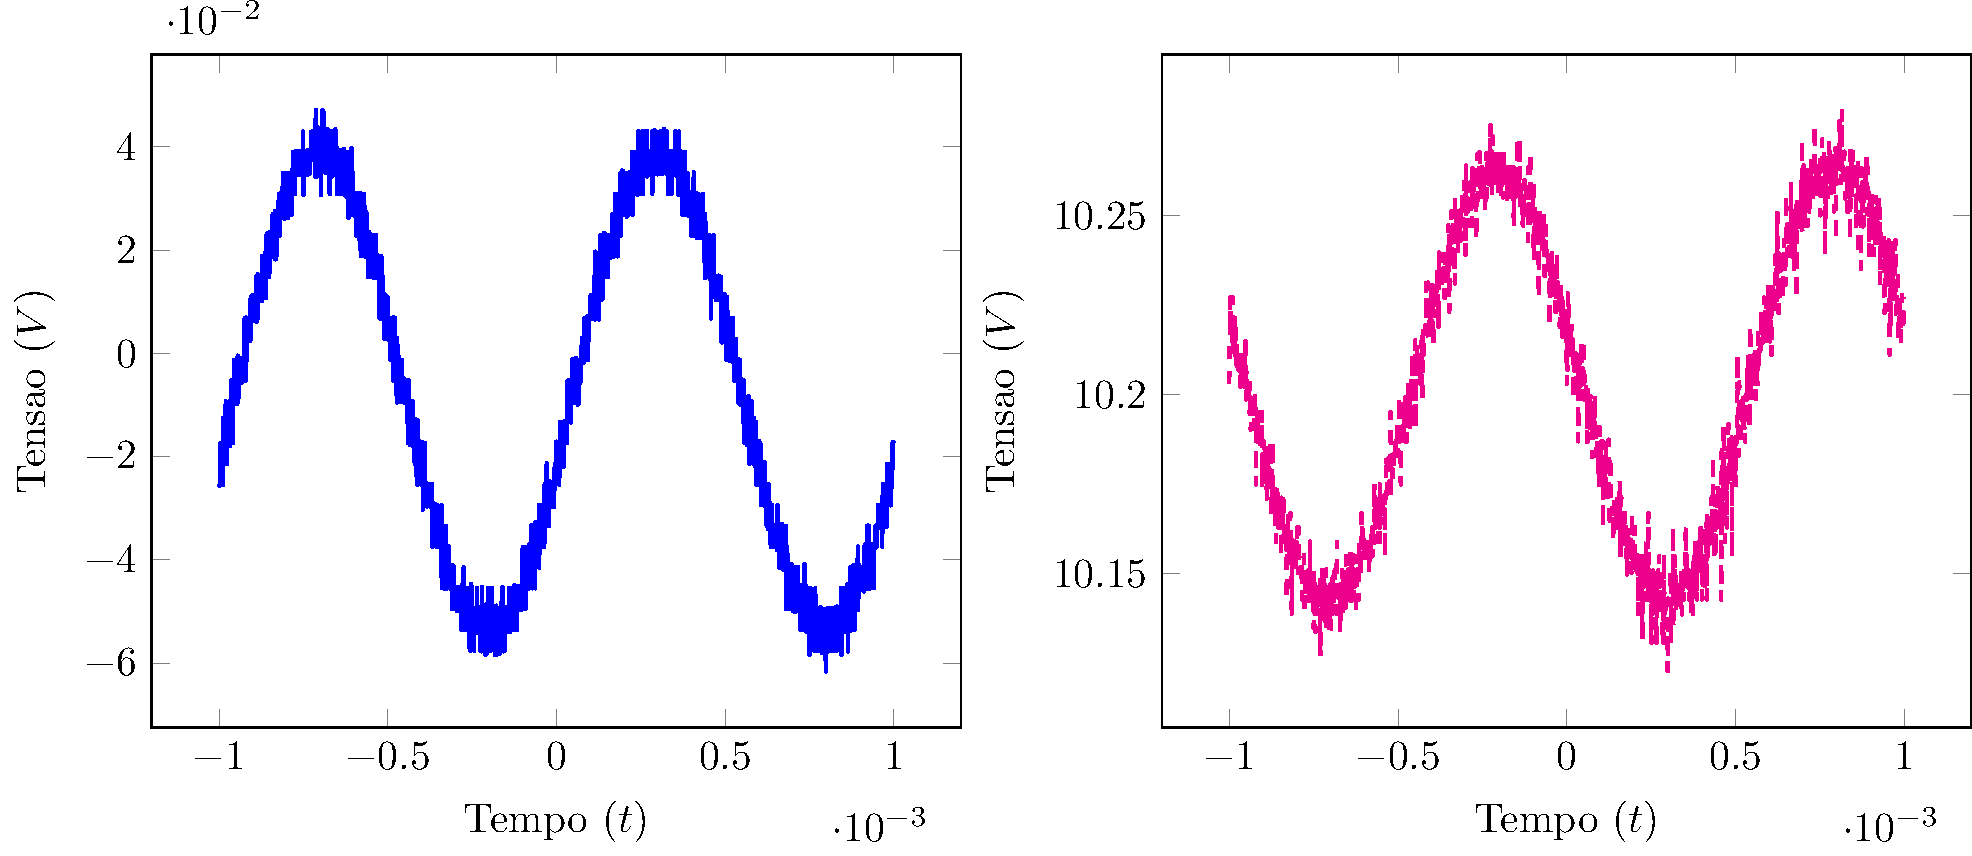
\includegraphics[width=\linewidth]{./img/scope2.pdf}
  \caption{Tensão de entrada (1Khz), em azul, e saída do circuito, em magenta, representado na Figura~1, com o capacitor desconectado. }
  \label{fig:degenerado}
\end{figure}

\subsection{Discussões}
Podemos então analizar a Tabela~2 para constatar que os valores de tensão  estimados e  empíricos parecem estar 
razoavelmente próximos, no entanto, constatamos, através da Tabela~2, que o ganho do circuito 
teórico e empírico são bem distantes. Isso ocorreu pois para o cálculo teórico utilizamos o valor de $I_{B_{Max}}$,
o que distorceu o ganho real do circuito. 
\begin{figure}[htpb]
  \centering
  \begin{tikzpicture}
    \begin{axis}[
      xlabel=$V_{CE}$,
      ylabel=$I_{C}$
      ]
      % use TeX as calculator:
      \addplot[color=magenta] coordinates {
        (0,0.015)
        (14.4,0)
      };
      \addplot [only marks,mark=*,blue] coordinates { 
        (6.23,0.00853) 
        (6.27,0.00842) 
        (6.39,0.00832) 
      };
    \end{axis}

  \end{tikzpicture}
  \caption{Reta de carga do circuito, com os pontos obtidos empiricamente graficados em azul .}
  \label{fig:carga}
\end{figure}
Para a entrada alternada de $10mV$ de pico , calculou-se os ganhos para o circuito não-degenerado e degenerado. Tais medidas foram
resumidas na Tabela~4. Este resultado é confirmado pelas nossas expectativas teóricas (advindas do modelo de pequenos sinais),
que dizem que sem o capacitor  de \emph{bypass} temos um circuito com baixo ganho.  Por fim , a reta de carga  mostrada na Figure~\ref{fig:carga}, enfatiza que os valores obtidos estão dentro do esperado, e 
que dada a reta de carga, podemos obter o valor da corrente através da queda da tensão no transistor e vice-versa.


\newpage
\subsection{Conclusão}
Primeiramente dimensionou-se  valores para os componentes do circuito para 
garantir-se o correto funcionamento da polarização do transistor. Dada estas 
condições, o circuito foi montado, com três transistores diferentes, e teve
seu ganho medido. A partir destas três medidas, pode-se comparar os ganhos
experimentais e teóricos e observou-se uma latente diferença entre as medidas 
empíricas e idealizadas.

Definida a polarização, aplicou-se um sinal de entrada de  baixa amplitude na
base do transistor, e observou-se a saída no coletor. Pôde-se então obter a 
relação entre  saída e entrada , seu ganho, tanto para o circuito degenerado e 
para o circuit não degenerado. Concluíu-se então que o capacitor de \emph{bypass}
é de suma importância para que o ganho do capacitor não se degrade.

Confirmou-se posteriormente a validade de nossas medidas
através da reta de carga. Concluindo assim, o experimento que mostra 
as condições de polarização automática de um $TBJ$, como adequar valores
ideais de componentes para valores comerciais, a possível grande diferença 
entre ganhos idealizados e obtidos empiracamente,  e o resultado que
releva a importância do capacitor de \emph{bypass}.
do \emph{bypass} 



\end{document}
